\section{Further directions for the project}
\label{sec4}


\subsection{Simple visualization methods}
\label{subsec41}

Sections \ref{sec2} and \ref{sec3} are dealing with interpretability topics that attracted much attention in recent research. Most of these methodologies use fairly sophisticated mathematical methods, and provide beautiful representations of neural networks and their activations. One particularly representative example of such methodology is the activation atlas methodology proposed by \cite{Carter2019}.

This method is sampling activations form many images, then summarizes the activations on the 2-D plan by using a reduction dimension of t-SNE or UMAP type, and averages over the saliency maps.

Figure \ref{im_sec4_1} provides an example of activation atlas :

\begin{figure}[H]
	\centering
	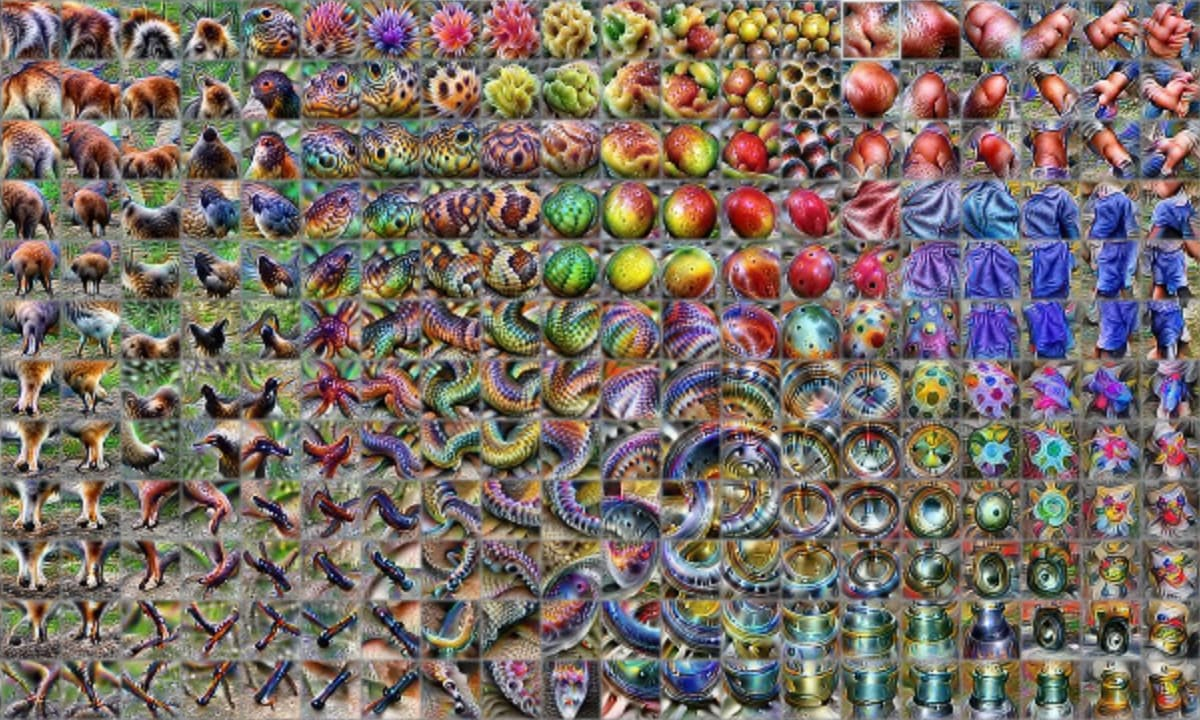
\includegraphics[width=\linewidth]{images/image2.png}
	\caption{An example of activation atlas}
	\label{im_sec4_1}
\end{figure}

While aesthetic, this representation may suffer from interpretation issues. Even though the goal of such methods is to render the network more interpretable, it is in fact quite difficult to conclude anything from such figure. To get more insights, one would need to read the paper carefully before and then look at the picture in much details to obtain useful information. For a professional with limited knowledge in neural networks, this sort of tools is probably not ideal.

On the other hand, simpler tools are being proposed in the recent literature. For instance, \cite{Peters2018} propose a more intuitive visualization method, specifically suitable for non-expert users. The method consists in representing neuron activation on a 2-D plan from a UMAP dimension reduction. In this respect, it is not so different in essence from the activation atlas. Yet the representation it provides is considerably simpler. Figure \ref{im_sec4_2} provides an example of this intuitive representation:

\begin{figure}[H]
	\centering
	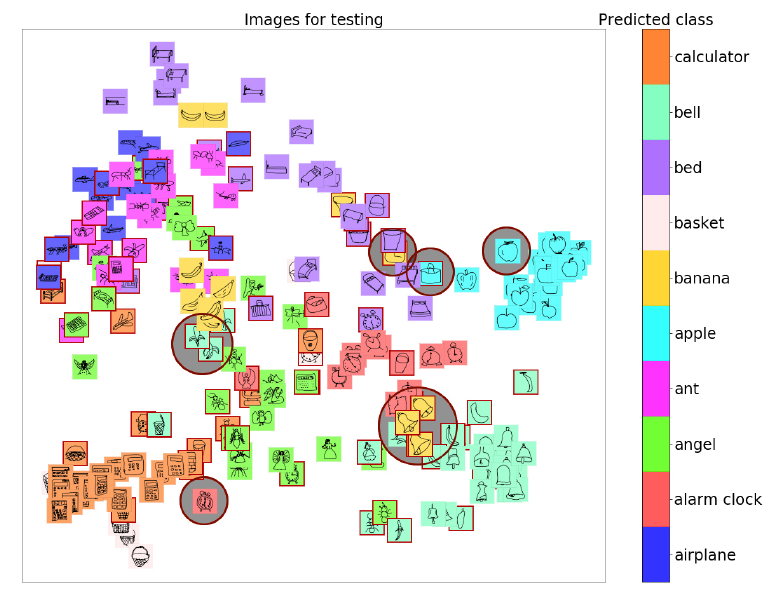
\includegraphics[width=\linewidth]{images/image5.png}
	\caption{An example of intuitive visualization}
	\label{im_sec4_2}
\end{figure}

The figure clearly discriminates the different classification categories using a palette of colors. Clustering highlights clearly which images are considered similar by the network, and miss-classified images are circled in red for immediate detection. This kind of representation does provide effective interpretation. Consider for instance the cluster of three bells on the lower-right side of the figure. These bells have been incorrectly classified as bananas, most likely because their diagonal orientation makes them closer to the other bananas than to their bell counterparts which can be seen to be in straight position.

In the end, when wondering which approach is the most informative, the second one would most likely be retained. This led our group to a real interrogation: what is the target audience for our visualization project? And what is the most suitable methodology to adopt to satisfy the needs of this audience? Should we adopt a sophisticated, state-of-the-art approach that may lead to technical performances and beautiful representations, or should we focus on simpler strategies that may in the end carry more immediate explanatory power? At the moment, we may be rather inclined to select the second solution, but this is yet a discussion to be pursued further.


\subsection{Future directions with the Minister of Armies}
\label{subsec42}

After discussion with the Ministère des Armées, we have decided to focus on the behavior of the neural network during the training. The adversarial training have been given up for our use case.
Our partner is willing to visualize how we could monitor the training through several metrics. We will deepen and extend all gradient-based and attribution technics for instance though the following metrics.
We have decided to proceeded along two mains axis :

Define following metrics : 
\begin{enumerate}
	\item Accuracy/loss during training and testing phasis, \cite{Glorot2010}, \cite{Li2017} 
	\item Evolution of gradients/weights for each epoch: cumulative differentiation between epochs to highlight DNN behavior and its main patterns, \cite{Chen2018}, \cite{Yosinski2015},  \cite{Rauber2016}, \cite{Cashman2019}
	\item Dynamic visualization of activations to observe the neural behavior and find neurons with similar or anti-similar behavior, \cite{Chen2018}, \cite{Yosinski2015}, \cite{Carter2019}
	\item Visualize the clustering evolution of main classes thanks to t-SNE or UMAP, \cite{Rauber2016} 
	\item Class discriminant features. \cite{Zintgraf2017}
	\item Provide an online tool to inspect the evolution of the deep neural network over epochs and given input samples.
\end{enumerate}

The final aim is to provide a proof of concept of some tools featuring different views based on previously listed metrics.  

